% This file was created by matlab2tikz.
%
%The latest updates can be retrieved from
%  http://www.mathworks.com/matlabcentral/fileexchange/22022-matlab2tikz-matlab2tikz
%where you can also make suggestions and rate matlab2tikz.
%
\definecolor{mycolor1}{rgb}{0.00000,0.44700,0.74100}%
%
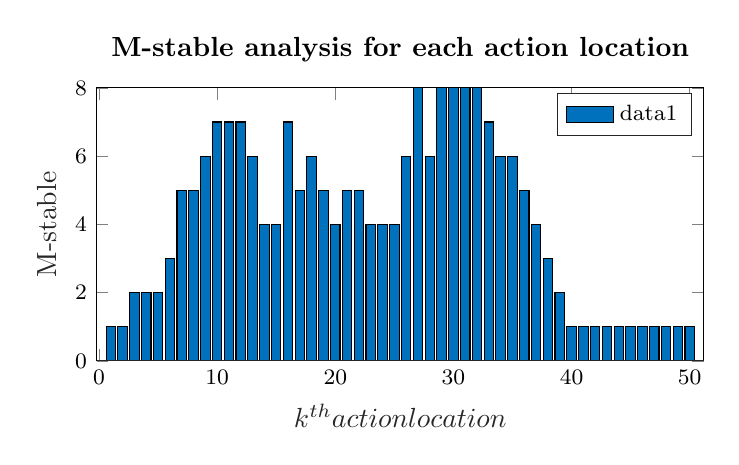
\begin{tikzpicture}

\begin{axis}[%
width=3.036in,
height=1.365in,
at={(0.677in,0.482in)},
scale only axis,
bar shift auto,
font=\footnotesize,
xmin=-0.2,
xmax=51.2,
xlabel style={font=\color{white!15!black}},
xlabel={$\text{k}^{\text{th}}\text{ action location}$},
ymin=0,
ymax=8,
ylabel style={font=\color{white!15!black}},
ylabel={M-stable},
axis background/.style={fill=white},
title style={font=\bfseries},
title={M-stable analysis for each action location},
legend style={legend cell align=left, align=left, draw=white!15!black}
]
\addplot[ybar, bar width=0.8, fill=mycolor1, draw=black, area legend] table[row sep=crcr] {%
1	1\\
2	1\\
3	2\\
4	2\\
5	2\\
6	3\\
7	5\\
8	5\\
9	6\\
10	7\\
11	7\\
12	7\\
13	6\\
14	4\\
15	4\\
16	7\\
17	5\\
18	6\\
19	5\\
20	4\\
21	5\\
22	5\\
23	4\\
24	4\\
25	4\\
26	6\\
27	8\\
28	6\\
29	8\\
30	8\\
31	8\\
32	8\\
33	7\\
34	6\\
35	6\\
36	5\\
37	4\\
38	3\\
39	2\\
40	1\\
41	1\\
42	1\\
43	1\\
44	1\\
45	1\\
46	1\\
47	1\\
48	1\\
49	1\\
50	1\\
};
\addplot[forget plot, color=white!15!black] table[row sep=crcr] {%
-0.2	0\\
51.2	0\\
};
\addlegendentry{data1}

\end{axis}
\end{tikzpicture}%